\documentclass{extbook}[14pt]
\usepackage{multicol, enumerate, enumitem, hyperref, color, soul, setspace, parskip, fancyhdr, amssymb, amsthm, amsmath, latexsym, units, mathtools}
\everymath{\displaystyle}
\usepackage[headsep=0.5cm,headheight=0cm, left=1 in,right= 1 in,top= 1 in,bottom= 1 in]{geometry}
\usepackage{dashrule}  % Package to use the command below to create lines between items
\newcommand{\litem}[1]{\item #1

\rule{\textwidth}{0.4pt}}
\pagestyle{fancy}
\lhead{}
\chead{Answer Key for Makeup Progress Quiz 2 Version B}
\rhead{}
\lfoot{2790-1423}
\cfoot{}
\rfoot{Summer C 2021}
\begin{document}
\textbf{This key should allow you to understand why you choose the option you did (beyond just getting a question right or wrong). \href{https://xronos.clas.ufl.edu/mac1105spring2020/courseDescriptionAndMisc/Exams/LearningFromResults}{More instructions on how to use this key can be found here}.}

\textbf{If you have a suggestion to make the keys better, \href{https://forms.gle/CZkbZmPbC9XALEE88}{please fill out the short survey here}.}

\textit{Note: This key is auto-generated and may contain issues and/or errors. The keys are reviewed after each exam to ensure grading is done accurately. If there are issues (like duplicate options), they are noted in the offline gradebook. The keys are a work-in-progress to give students as many resources to improve as possible.}

\rule{\textwidth}{0.4pt}

\begin{enumerate}\litem{
Which of the following equations \textit{could} be of the graph presented below?

\begin{center}
    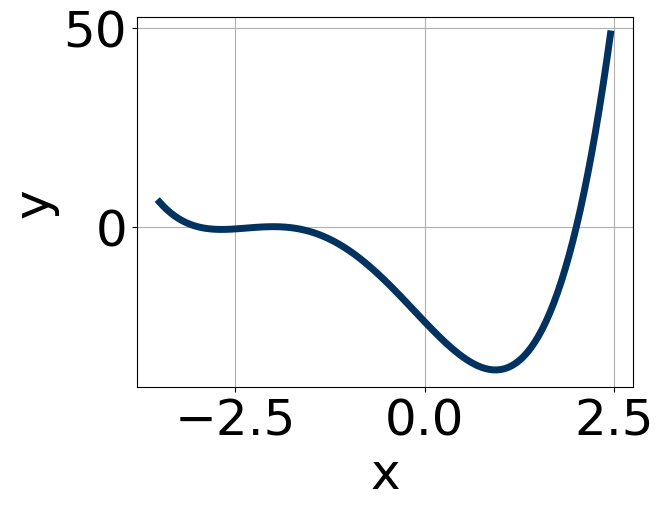
\includegraphics[width=0.5\textwidth]{../Figures/polyGraphToFunctionB.png}
\end{center}


The solution is \( 13(x + 2)^{4} (x - 2)^{11} (x + 3)^{11} \), which is option C.\begin{enumerate}[label=\Alph*.]
\item \( 19(x + 2)^{7} (x - 2)^{4} (x + 3)^{9} \)

The factor $-2$ should have an even power and the factor $2$ should have an odd power.
\item \( 20(x + 2)^{10} (x - 2)^{8} (x + 3)^{7} \)

The factor $(x - 2)$ should have an odd power.
\item \( 13(x + 2)^{4} (x - 2)^{11} (x + 3)^{11} \)

* This is the correct option.
\item \( -18(x + 2)^{4} (x - 2)^{7} (x + 3)^{4} \)

The factor $(x + 3)$ should have an odd power and the leading coefficient should be the opposite sign.
\item \( -4(x + 2)^{10} (x - 2)^{11} (x + 3)^{5} \)

This corresponds to the leading coefficient being the opposite value than it should be.
\end{enumerate}

\textbf{General Comment:} General Comments: Draw the x-axis to determine which zeros are touching (and so have even multiplicity) or cross (and have odd multiplicity).
}
\litem{
Construct the lowest-degree polynomial given the zeros below. Then, choose the intervals that contain the coefficients of the polynomial in the form $ax^3+bx^2+cx+d$.
\[ \frac{1}{4}, \frac{7}{5}, \text{ and } 2 \]The solution is \( 20x^{3} -73 x^{2} +73 x -14 \), which is option C.\begin{enumerate}[label=\Alph*.]
\item \( a \in [17, 26], b \in [68, 75], c \in [69, 74], \text{ and } d \in [10, 16] \)

$20x^{3} +73 x^{2} +73 x + 14$, which corresponds to multiplying out $(4x + 1)(5x + 7)(x + 2)$.
\item \( a \in [17, 26], b \in [-7, -6], c \in [-59, -56], \text{ and } d \in [-18, -13] \)

$20x^{3} -7 x^{2} -59 x -14$, which corresponds to multiplying out $(4x + 1)(5x + 7)(x -2)$.
\item \( a \in [17, 26], b \in [-73, -66], c \in [69, 74], \text{ and } d \in [-18, -13] \)

* $20x^{3} -73 x^{2} +73 x -14$, which is the correct option.
\item \( a \in [17, 26], b \in [-73, -66], c \in [69, 74], \text{ and } d \in [10, 16] \)

$20x^{3} -73 x^{2} +73 x + 14$, which corresponds to multiplying everything correctly except the constant term.
\item \( a \in [17, 26], b \in [-66, -58], c \in [34, 45], \text{ and } d \in [10, 16] \)

$20x^{3} -63 x^{2} +39 x + 14$, which corresponds to multiplying out $(4x + 1)(5x -7)(x -2)$.
\end{enumerate}

\textbf{General Comment:} To construct the lowest-degree polynomial, you want to multiply out $(4x -1)(5x -7)(x -2)$
}
\litem{
Describe the zero behavior of the zero $x = 2$ of the polynomial below.
\[ f(x) = -9(x - 7)^{7}(x + 7)^{4}(x - 2)^{12}(x + 2)^{9} \]The solution is the graph below, which is option C.
    \begin{center}
        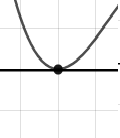
\includegraphics[width=0.3\textwidth]{../Figures/polyZeroBehaviorCopyCB.png}
    \end{center}\begin{enumerate}[label=\Alph*.]
\begin{multicols}{2}
\item 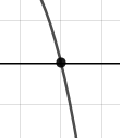
\includegraphics[width = 0.3\textwidth]{../Figures/polyZeroBehaviorCopyAB.png}
\item 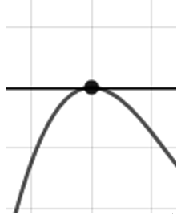
\includegraphics[width = 0.3\textwidth]{../Figures/polyZeroBehaviorCopyBB.png}
\item 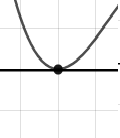
\includegraphics[width = 0.3\textwidth]{../Figures/polyZeroBehaviorCopyCB.png}
\item 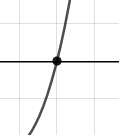
\includegraphics[width = 0.3\textwidth]{../Figures/polyZeroBehaviorCopyDB.png}
\end{multicols}\item None of the above.\end{enumerate}
\textbf{General Comment:} You will need to sketch the entire graph, then zoom in on the zero the question asks about.
}
\litem{
Describe the end behavior of the polynomial below.
\[ f(x) = 8(x - 9)^{2}(x + 9)^{5}(x - 7)^{4}(x + 7)^{6} \]The solution is the graph below, which is option D.
    \begin{center}
        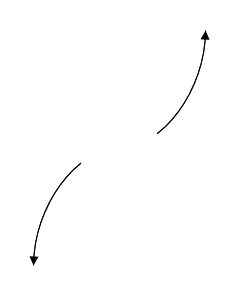
\includegraphics[width=0.3\textwidth]{../Figures/polyEndBehaviorCopyDB.png}
    \end{center}\begin{enumerate}[label=\Alph*.]
\begin{multicols}{2}
\item 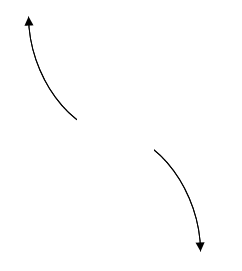
\includegraphics[width = 0.3\textwidth]{../Figures/polyEndBehaviorCopyAB.png}
\item 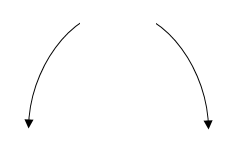
\includegraphics[width = 0.3\textwidth]{../Figures/polyEndBehaviorCopyBB.png}
\item 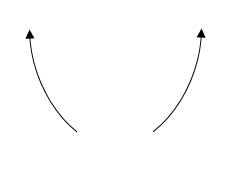
\includegraphics[width = 0.3\textwidth]{../Figures/polyEndBehaviorCopyCB.png}
\item 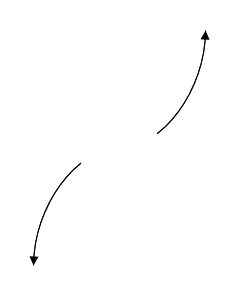
\includegraphics[width = 0.3\textwidth]{../Figures/polyEndBehaviorCopyDB.png}
\end{multicols}\item None of the above.\end{enumerate}
\textbf{General Comment:} Remember that end behavior is determined by the leading coefficient AND whether the \textbf{sum} of the multiplicities is positive or negative.
}
\litem{
Describe the end behavior of the polynomial below.
\[ f(x) = 9(x + 5)^{3}(x - 5)^{6}(x - 3)^{5}(x + 3)^{7} \]The solution is the graph below, which is option D.
    \begin{center}
        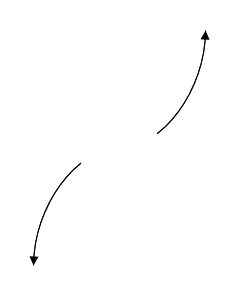
\includegraphics[width=0.3\textwidth]{../Figures/polyEndBehaviorDB.png}
    \end{center}\begin{enumerate}[label=\Alph*.]
\begin{multicols}{2}
\item 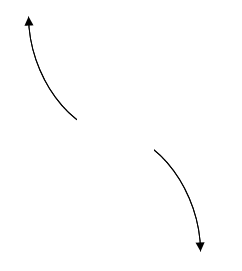
\includegraphics[width = 0.3\textwidth]{../Figures/polyEndBehaviorAB.png}
\item 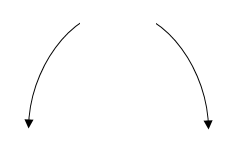
\includegraphics[width = 0.3\textwidth]{../Figures/polyEndBehaviorBB.png}
\item 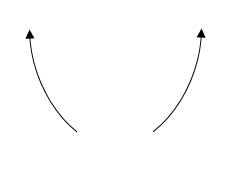
\includegraphics[width = 0.3\textwidth]{../Figures/polyEndBehaviorCB.png}
\item 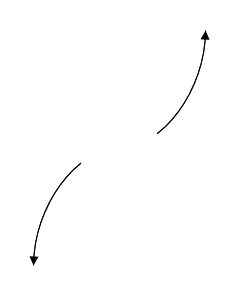
\includegraphics[width = 0.3\textwidth]{../Figures/polyEndBehaviorDB.png}
\end{multicols}\item None of the above.\end{enumerate}
\textbf{General Comment:} Remember that end behavior is determined by the leading coefficient AND whether the \textbf{sum} of the multiplicities is positive or negative.
}
\litem{
Construct the lowest-degree polynomial given the zeros below. Then, choose the intervals that contain the coefficients of the polynomial in the form $x^3+bx^2+cx+d$.
\[ -2 + 5 i \text{ and } 3 \]The solution is \( x^{3} + x^{2} +17 x -87 \), which is option A.\begin{enumerate}[label=\Alph*.]
\item \( b \in [-0.1, 2.4], c \in [15, 24], \text{ and } d \in [-94, -80] \)

* $x^{3} + x^{2} +17 x -87$, which is the correct option.
\item \( b \in [-2.5, -0.9], c \in [15, 24], \text{ and } d \in [75, 89] \)

$x^{3} -1 x^{2} +17 x + 87$, which corresponds to multiplying out $(x-(-2 + 5 i))(x-(-2 - 5 i))(x + 3)$.
\item \( b \in [-0.1, 2.4], c \in [-8, -3], \text{ and } d \in [10, 24] \)

$x^{3} + x^{2} -8 x + 15$, which corresponds to multiplying out $(x -5)(x -3)$.
\item \( b \in [-0.1, 2.4], c \in [-2, 5], \text{ and } d \in [-10, -2] \)

$x^{3} + x^{2} -x -6$, which corresponds to multiplying out $(x + 2)(x -3)$.
\item \( \text{None of the above.} \)

This corresponds to making an unanticipated error or not understanding how to use nonreal complex numbers to create the lowest-degree polynomial. If you chose this and are not sure what you did wrong, please contact the coordinator for help.
\end{enumerate}

\textbf{General Comment:} Remember that the conjugate of $a+bi$ is $a-bi$. Since these zeros always come in pairs, we need to multiply out $(x-(-2 + 5 i))(x-(-2 - 5 i))(x-(3))$.
}
\litem{
Construct the lowest-degree polynomial given the zeros below. Then, choose the intervals that contain the coefficients of the polynomial in the form $ax^3+bx^2+cx+d$.
\[ \frac{-3}{2}, \frac{-7}{3}, \text{ and } -4 \]The solution is \( 6x^{3} +47 x^{2} +113 x + 84 \), which is option D.\begin{enumerate}[label=\Alph*.]
\item \( a \in [1, 13], b \in [42, 51], c \in [111, 117], \text{ and } d \in [-87, -83] \)

$6x^{3} +47 x^{2} +113 x -84$, which corresponds to multiplying everything correctly except the constant term.
\item \( a \in [1, 13], b \in [-4, 2], c \in [-76, -68], \text{ and } d \in [84, 88] \)

$6x^{3} + x^{2} -71 x + 84$, which corresponds to multiplying out $(2x -3)(3x -7)(x + 4)$.
\item \( a \in [1, 13], b \in [-50, -41], c \in [111, 117], \text{ and } d \in [-87, -83] \)

$6x^{3} -47 x^{2} +113 x -84$, which corresponds to multiplying out $(2x -3)(3x -7)(x -4)$.
\item \( a \in [1, 13], b \in [42, 51], c \in [111, 117], \text{ and } d \in [84, 88] \)

* $6x^{3} +47 x^{2} +113 x + 84$, which is the correct option.
\item \( a \in [1, 13], b \in [28, 30], c \in [-3, 5], \text{ and } d \in [-87, -83] \)

$6x^{3} +29 x^{2} -x -84$, which corresponds to multiplying out $(2x -3)(3x + 7)(x + 4)$.
\end{enumerate}

\textbf{General Comment:} To construct the lowest-degree polynomial, you want to multiply out $(2x + 3)(3x + 7)(x + 4)$
}
\litem{
Which of the following equations \textit{could} be of the graph presented below?

\begin{center}
    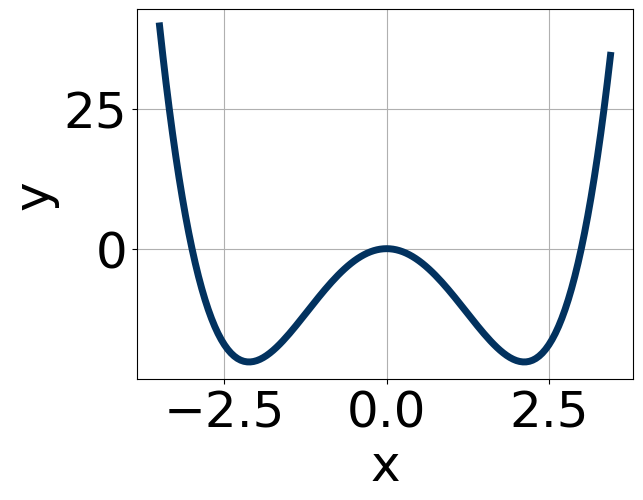
\includegraphics[width=0.5\textwidth]{../Figures/polyGraphToFunctionCopyB.png}
\end{center}


The solution is \( 18x^{8} (x + 3)^{9} (x - 3)^{7} \), which is option A.\begin{enumerate}[label=\Alph*.]
\item \( 18x^{8} (x + 3)^{9} (x - 3)^{7} \)

* This is the correct option.
\item \( -19x^{4} (x + 3)^{5} (x - 3)^{4} \)

The factor $(x - 3)$ should have an odd power and the leading coefficient should be the opposite sign.
\item \( 19x^{4} (x + 3)^{8} (x - 3)^{11} \)

The factor $(x + 3)$ should have an odd power.
\item \( 8x^{5} (x + 3)^{8} (x - 3)^{7} \)

The factor $0$ should have an even power and the factor $-3$ should have an odd power.
\item \( -3x^{4} (x + 3)^{11} (x - 3)^{7} \)

This corresponds to the leading coefficient being the opposite value than it should be.
\end{enumerate}

\textbf{General Comment:} General Comments: Draw the x-axis to determine which zeros are touching (and so have even multiplicity) or cross (and have odd multiplicity).
}
\litem{
Construct the lowest-degree polynomial given the zeros below. Then, choose the intervals that contain the coefficients of the polynomial in the form $x^3+bx^2+cx+d$.
\[ 5 + 2 i \text{ and } 4 \]The solution is \( x^{3} -14 x^{2} +69 x -116 \), which is option B.\begin{enumerate}[label=\Alph*.]
\item \( b \in [-6, 2], c \in [-9.4, -7.5], \text{ and } d \in [18, 22] \)

$x^{3} + x^{2} -9 x + 20$, which corresponds to multiplying out $(x -5)(x -4)$.
\item \( b \in [-21, -8], c \in [67.5, 70.9], \text{ and } d \in [-126, -113] \)

* $x^{3} -14 x^{2} +69 x -116$, which is the correct option.
\item \( b \in [-6, 2], c \in [-8, -3.8], \text{ and } d \in [5, 12] \)

$x^{3} + x^{2} -6 x + 8$, which corresponds to multiplying out $(x -2)(x -4)$.
\item \( b \in [12, 21], c \in [67.5, 70.9], \text{ and } d \in [115, 119] \)

$x^{3} +14 x^{2} +69 x + 116$, which corresponds to multiplying out $(x-(5 + 2 i))(x-(5 - 2 i))(x + 4)$.
\item \( \text{None of the above.} \)

This corresponds to making an unanticipated error or not understanding how to use nonreal complex numbers to create the lowest-degree polynomial. If you chose this and are not sure what you did wrong, please contact the coordinator for help.
\end{enumerate}

\textbf{General Comment:} Remember that the conjugate of $a+bi$ is $a-bi$. Since these zeros always come in pairs, we need to multiply out $(x-(5 + 2 i))(x-(5 - 2 i))(x-(4))$.
}
\litem{
Describe the zero behavior of the zero $x = 2$ of the polynomial below.
\[ f(x) = 8(x + 2)^{2}(x - 2)^{7}(x - 4)^{9}(x + 4)^{11} \]The solution is the graph below, which is option A.
    \begin{center}
        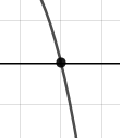
\includegraphics[width=0.3\textwidth]{../Figures/polyZeroBehaviorAB.png}
    \end{center}\begin{enumerate}[label=\Alph*.]
\begin{multicols}{2}
\item 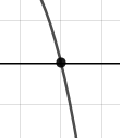
\includegraphics[width = 0.3\textwidth]{../Figures/polyZeroBehaviorAB.png}
\item 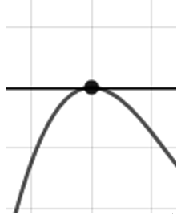
\includegraphics[width = 0.3\textwidth]{../Figures/polyZeroBehaviorBB.png}
\item 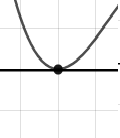
\includegraphics[width = 0.3\textwidth]{../Figures/polyZeroBehaviorCB.png}
\item 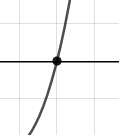
\includegraphics[width = 0.3\textwidth]{../Figures/polyZeroBehaviorDB.png}
\end{multicols}\item None of the above.\end{enumerate}
\textbf{General Comment:} You will need to sketch the entire graph, then zoom in on the zero the question asks about.
}
\end{enumerate}

\end{document}